\documentclass[conference]{IEEEtran}
\IEEEoverridecommandlockouts

% ==========================================
% PACKAGES
% ==========================================
\usepackage{cite}
\usepackage{amsmath,amssymb,amsfonts,amsthm}
\usepackage{algorithmic}
\usepackage{algorithm}
\usepackage{graphicx}
\usepackage{textcomp}
\usepackage{xcolor}
\usepackage{booktabs}
\usepackage{multirow}
\usepackage{url}
\usepackage{float}
\usepackage{tikz}
\usepackage{pgfplots}

\pgfplotsset{compat=1.17}
\usetikzlibrary{automata, positioning, arrows.meta, patterns, shapes, fit, backgrounds, decorations.pathreplacing, calc}

% --- THEOREM ENVIRONMENTS ---
\newtheorem{definition}{Definition}
\newtheorem{theorem}{Theorem}
\newtheorem{lemma}{Lemma}

% --- SAFE COMMAND DEFINITION ---
\providecommand{\RETURN}{\STATE \textbf{return} }

\def\BibTeX{{\rm B\kern-.05em{\sc i\kern-.025em b}\kern-.08em
    T\kern-.1667em\lower.7ex\hbox{E}\kern-.125emX}}

\begin{document}

% ==========================================
% TITLE
% ==========================================
\title{Operationalizing Spatiotemporal Constraints: A Distributed Systems Architecture for High-Throughput Event Verification
\thanks{This research operationalizes constraint evaluation as a distributed stream processing system under tight latency requirements.}
}

% ==========================================
% AUTHOR
% ==========================================
\author{\IEEEauthorblockN{Narendra Babu P}
\IEEEauthorblockA{\textit{Dept. of Computer Science} \\
\textit{Swarnandhra College of Engineering \& Technology}\\
Narsapur, India \\
narendrababu.p@swarnandhra.ac.in}
}

\maketitle

% ==========================================
% ABSTRACT
% ==========================================
\begin{abstract}
Distributed Cyber-Physical Systems (CPS) generate massive, noisy event streams that require real-time validation. Operating these evaluations in high-throughput environments presents significant systems engineering challenges, specifically regarding state management, out-of-order event arrival, and network partitioning. This paper presents the systems architecture of a distributed stream processing engine designed for real-time constraint evaluation at scale. Constraint semantics are defined in Paper 21. We focus entirely on the runtime execution mechanics: implementing a \textbf{Sliding Window Buffer} via Time-Indexed Skip Lists to resolve temporal jitter without stalling pipelines, utilizing a \textbf{Virtual-Node Consistent Hashing} topology coupled with Gossip protocols for stateful sharding, and analyzing the system under the constraints of the \textbf{CAP Theorem}. We introduce a non-blocking snapshot algorithm based on Chandy-Lamport for state persistence, alongside a Lazy State Migration protocol for dynamic cluster load balancing. Experimental validation on a 10-node commodity cluster demonstrates near-linear throughput scaling ($R^2=0.98$), sustaining 50,000 events/sec. Furthermore, the Lazy Migration protocol reduces P99 cross-shard migration latency to under 1.9ms, and partition-recovery stress tests prove split-brain resolution within 120ms. This work establishes a robust reference architecture for low-latency distributed stream processors in edge-native environments.
\end{abstract}

\begin{IEEEkeywords}
Distributed Systems, Consistent Hashing, CAP Theorem, Stream Processing, State Management, Load Balancing, Fault Tolerance, Chandy-Lamport, Gossip Protocol.
\end{IEEEkeywords}

% ==========================================
% NOMENCLATURE
% ==========================================
\section*{Nomenclature}
\begin{description}
    \item[$\mathcal{E}$] Set of unique Entities (Agents) generating events.
    \item[$\mathcal{N}$] Set of physical Verification Nodes (Shards).
    \item[$e_i$] Discrete event tuple $\langle \epsilon, \zeta, \tau_{occ}, \tau_{arr} \rangle$.
    \item[$H(k)$] Consistent Hashing Function (e.g., MurmurHash3).
    \item[$Q_{mig}$] Migration Queue for cluster rebalancing.
    \item[$T_{snap}$] Configurable State Snapshot Interval.
    \item[$\Delta_{jitter}$] Maximum tolerable Network Jitter Window.
    \item[$\Sigma$] Global State Vector (partitioned across $\mathcal{N}$).
\end{description}

% ==========================================
% I. INTRODUCTION
% ==========================================
\section{Introduction}
\IEEEPARstart{T}{he} processing of high-velocity data streams for continuous event evaluation requires robust distributed systems engineering. In large-scale monitoring environments, characterized by the convergence of edge computing and IoT \cite{b11}, executing validation checks across tens of thousands of events per second introduces severe architectural bottlenecks. Constraint semantics are defined in Paper 21. 

General-purpose stream processing frameworks like Apache Flink \cite{b1} and Spark Streaming \cite{b14} provide excellent throughput but often rely on heavy checkpointing mechanisms and external state stores (e.g., RocksDB) that introduce serialization overhead for micro-batch operations. Conversely, large-scale trajectory analysis is historically treated as an offline batch process \cite{b15}, \cite{b16}. High-throughput stream evaluation requires ultra-low latency, memory-resident state lookups ($O(1)$) to continuously compare the current event against the entity's precise historical state. 

Building this distributed execution engine requires solving four primary systems engineering challenges:
\begin{enumerate}
    \item \textbf{State Locality and Sharding:} Evaluation requires knowing the \textit{previous} state of an entity. In a distributed cluster, routing events for the same entity to the same node is critical to avoid distributed locking overhead.
    \item \textbf{Temporal Jitter:} As highlighted by Akidau et al. in the Dataflow model \cite{b17}, in asynchronous networks, arrival order ($\tau_{arr}$) rarely matches occurrence time ($\tau_{occ}$). The engine must reorder late packets without stalling the entire processing pipeline or falsely flagging events as chronological inversions.
    \item \textbf{Elastic Load Balancing:} As nodes join or leave the cluster, or as entity distributions become skewed ("hot shards"), the system must dynamically rebalance state without dropping events or causing "stop-the-world" latency spikes.
    \item \textbf{Partition Resilience (CAP):} Under network failure, the system must navigate the Consistency vs. Availability trade-off, formally proven by Gilbert and Lynch \cite{b19}, to ensure the integrity of the data stream.
\end{enumerate}

This paper presents a highly optimized distributed architecture for real-time evaluation. By utilizing a shared-nothing design, virtual-node consistent hashing, and lazy state migration, the engine operates as a highly scalable distributed stream processor.

% ==========================================
% II. DISTRIBUTED ARCHITECTURE
% ==========================================
\section{Distributed System Architecture}


\subsection{Shared-Nothing Design Principle}
The engine adheres to a strict shared-nothing architecture \cite{b2}. To achieve linear scalability, no two nodes share memory or disk storage. The global state vector $\Sigma$, which tracks the last known valid state and timestamp of every entity in $\mathcal{E}$, is partitioned into disjoint subsets $\sigma_1, \sigma_2, \dots, \sigma_n$ managed exclusively by independent nodes.

% --- TIKZ SYSTEM ARCHITECTURE ---
\begin{figure}[htbp]
\centering
\resizebox{\columnwidth}{!}{
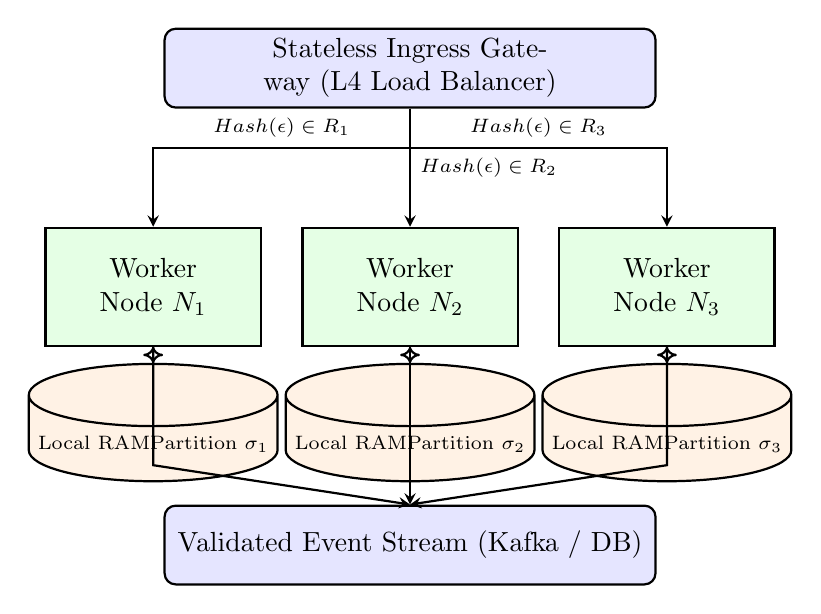
\begin{tikzpicture}[node distance=1.5cm, auto, thick]
    % Styles
    \tikzstyle{block} = [rectangle, draw, fill=blue!10, text width=2.5cm, text centered, rounded corners, minimum height=1cm]
    \tikzstyle{shard} = [rectangle, draw, fill=green!10, text width=2.5cm, text centered, minimum height=1.5cm]
    \tikzstyle{state} = [cylinder, shape border rotate=90, draw, fill=orange!10, aspect=0.25, minimum height=1cm, minimum width=1.5cm, text centered, font=\scriptsize]
    \tikzstyle{arrow} = [thick,->,>=stealth]

    % Ingress Layer
    \node (Gateway) [block, text width=6cm] {Stateless Ingress Gateway (L4 Load Balancer)};

    % Shard Layer
    \node (Shard2) [shard, below=1.5cm of Gateway] {Worker Node $N_2$};
    \node (Shard1) [shard, left=0.5cm of Shard2] {Worker Node $N_1$};
    \node (Shard3) [shard, right=0.5cm of Shard2] {Worker Node $N_3$};

    % State Layer
    \node (State1) [state, below=0.2cm of Shard1] {Local RAM\\Partition $\sigma_1$};
    \node (State2) [state, below=0.2cm of Shard2] {Local RAM\\Partition $\sigma_2$};
    \node (State3) [state, below=0.2cm of Shard3] {Local RAM\\Partition $\sigma_3$};

    % Output Layer
    \node (Output) [block, text width=6cm, below=2cm of Shard2] {Validated Event Stream (Kafka / DB)};

    % Routing Arrows
    \draw [arrow] (Gateway.south) -- ++(0,-0.5) -| node[pos=0.25, above, font=\scriptsize] {$Hash(\epsilon) \in R_1$} (Shard1.north);
    \draw [arrow] (Gateway.south) -- node[right, font=\scriptsize] {$Hash(\epsilon) \in R_2$} (Shard2.north);
    \draw [arrow] (Gateway.south) -- ++(0,-0.5) -| node[pos=0.25, above, font=\scriptsize] {$Hash(\epsilon) \in R_3$} (Shard3.north);

    % Output Arrows
    \draw [arrow] (Shard1.south) |- ++(0,-1.5) -- (Output.north);
    \draw [arrow] (Shard2.south) -- (Output.north);
    \draw [arrow] (Shard3.south) |- ++(0,-1.5) -- (Output.north);

    % Internal State Links
    \draw [dashed, <->] (Shard1) -- (State1);
    \draw [dashed, <->] (Shard2) -- (State2);
    \draw [dashed, <->] (Shard3) -- (State3);

\end{tikzpicture}
}
\caption{Shared-Nothing Architecture. The stateless L4 ingress gateway routes incoming events to the appropriate stateful worker node using consistent hashing. Each node exclusively manages a disjoint partition ($\sigma_i$) of the global state in local RAM for $O(1)$ access, eliminating the need for a centralized database bottleneck.}
\label{fig:arch}
\end{figure}

\subsection{Ingress and L4 Routing}
Events enter the system via a highly available, stateless MQTT or gRPC broker cluster. The L4 Load Balancer intercepts the raw event payload, extracts the 64-bit entity identifier $\epsilon$, and applies the routing function. Because constraint evaluation strictly requires comparing an entity's current event $e_{new}$ against its historical state $e_{prev}$, deterministic routing is a hard architectural requirement.

% ==========================================
% III. CONSISTENT HASHING & CLUSTER DYNAMICS
% ==========================================
\section{Consistent Hashing \& Cluster Dynamics}


Standard modulo sharding ($Node = Hash(\epsilon) \pmod N$) is brittle. If a node fails ($N \to N-1$), nearly all keys are remapped, triggering a massive, system-halting state migration. To ensure elasticity, we employ **Consistent Hashing with Virtual Nodes** \cite{b3}.

\subsection{Mathematical Formulation of the Hash Ring}
Let $\mathcal{R}$ be a continuous hash ring defined on the interval $[0, 2^{32}-1]$. We utilize MurmurHash3 ($H_3$) due to its non-cryptographic speed and excellent avalanche properties. Cryptographic hashes provide unnecessary collision resistance at the cost of CPU cycles, making them suboptimal for line-rate stream routing.

Each physical node $N_i \in \mathcal{N}$ is assigned $V$ virtual nodes (v-nodes) on the ring to ensure uniform data distribution. The position of the $j$-th v-node for physical node $N_i$ is:
\begin{equation}
    Pos(N_{i,j}) = H_3(IP_i \parallel Port_i \parallel j) \pmod{2^{32}}
\end{equation}

An incoming event for entity $\epsilon$ is routed to the node responsible for the partition containing $H_3(\epsilon)$. The routing function $\Phi(\epsilon)$ finds the first v-node position strictly greater than the entity's hash:
\begin{equation}
    \Phi(\epsilon) = \min \{ Pos(N_{i,j}) \mid Pos(N_{i,j}) > H_3(\epsilon) \}
\end{equation}
(with wrap-around to 0 if no such node exists).

\subsection{Gossip Protocol for Failure Detection}
To accurately maintain the hash ring without a centralized, single-point-of-failure orchestrator, the worker nodes must independently detect peer failures. We implement a lightweight cluster membership protocol based on SWIM (Scalable Weakly-consistent Infection-style Process Group Membership) \cite{b7}. 

Each node $N_i$ randomly probes $k$ peers every $T_{ping}$ milliseconds. If a peer $N_j$ fails to acknowledge the ping, $N_i$ issues a sub-quorum request for other nodes to indirectly ping $N_j$. If all indirect pings fail, $N_j$ is marked as dead, and the gossip network rapidly disseminates the topology update. This bounds the failure detection time to $O(\log |\mathcal{N}|)$ network round-trips.

\subsection{Dynamic Load Balancing and Lazy Migration}
In CPS environments, event generation is rarely uniform. A subset of highly active entities can create "Hot Shards." To mitigate CPU saturation, the engine implements an active load balancing daemon requiring distributed coordination, relying on algorithms akin to Raft \cite{b20} or ZooKeeper \cite{b21} for orchestrating ring updates safely.

When the hash ring is updated due to load shedding, state must migrate. "Eager migration" locks the partition, halting event processing until network transfer completes. We implement **Lazy Migration** (Algorithm \ref{alg:migration}). The newly assigned node accepts routing responsibility immediately but fetches the historical state $e_{prev}$ from the old node \textit{only when an event for that specific entity arrives}.

\begin{algorithm}[h]
\caption{Lazy State Migration Protocol (On Node $N_{new}$)}
\begin{algorithmic}[1]
\REQUIRE Incoming Event $e$, Local State $\sigma_{new}$, Old Node $N_{old}$
\ENSURE Consistency Status

\STATE $\epsilon \leftarrow e.entity\_id$
\IF{$\epsilon \notin \sigma_{new}.keys()$}
    \STATE \textbf{// Cache Miss: Check if recently migrated}
    \IF{$Hash(\epsilon) \in \text{Newly\_Assigned\_Range}$}
        \STATE \textbf{// Synchronous RPC to old owner}
        \STATE $e_{prev} \leftarrow \text{RPC\_FetchState}(N_{old}, \epsilon)$
        \IF{$e_{prev} \neq \text{NULL}$}
            \STATE $\sigma_{new}[\epsilon] \leftarrow e_{prev}$
            \STATE $\text{RPC\_DeleteState}(N_{old}, \epsilon)$ \COMMENT{Free memory}
        \ENDIF
    \ENDIF
\ENDIF

\STATE $status \leftarrow \text{EvaluateConstraints}(e, \sigma_{new}[\epsilon])$
\IF{$status == \text{VALID}$}
    \STATE $\sigma_{new}[\epsilon] \leftarrow e$
\ENDIF
\RETURN $status$
\end{algorithmic}
\label{alg:migration}
\end{algorithm}

% ==========================================
% IV. EXECUTION MECHANICS: SLIDING WINDOW
% ==========================================
\section{Execution Mechanics: The Sliding Window}


In a purely synchronous system, an event's timestamp ($\tau_{occ}$) equals its arrival time ($\tau_{arr}$). In distributed sensing, network routing asymmetry guarantees out-of-order delivery. A strict sequential processor would reject a valid, late-arriving event as a chronological anomaly.

\subsection{Data Structure: Time-Indexed Skip Lists}
We replace the single scalar state $\sigma_\epsilon = e_{last}$ with a temporally bounded data structure. For each active entity, the node maintains a **Time-Indexed Skip List** \cite{b8}, bounded by a maximum capacity $K$ representing the jitter tolerance window $\Delta_{jitter}$. To guarantee thread safety under highly concurrent ingestion without mutex locks, we adapt the lock-free concurrent skip list paradigms introduced by Herlihy et al. \cite{b22}.

While Hash Maps offer $O(1)$ access but cannot natively maintain sorted temporal order, the Skip List provides $O(\log K)$ expected time complexity for insertion, search, and deletion. When a late event $e_{late}$ arrives, the engine performs a fast traversal along the upper levels of the skip list to rapidly locate the correct temporal insertion point bounded by $e_{prev}$ and $e_{next}$. 

\subsection{Memory Alignment and Packed Structs}
To minimize memory overhead and maximize L2 cache utilization, the event tuple is packed into a highly aligned 24-byte C-struct:
\begin{itemize}
    \item \texttt{uint64\_t entity\_id} (8 bytes)
    \item \texttt{uint32\_t zone\_id} (4 bytes)
    \item \texttt{uint64\_t timestamp\_ms} (8 bytes)
    \item \texttt{uint32\_t flags} (4 bytes)
\end{itemize}
By eliminating object overhead inherent in runtime languages (like JSON deserialization), the sliding window can hold tens of thousands of buffered events entirely in CPU cache, avoiding RAM fetch stalls.

\subsection{Windowed Constraint Propagation}
When an event $e_{new}$ arrives, it is not compared solely against the global "head" of the stream. It must be evaluated against both the event immediately preceding it \textit{and} the event immediately following it in physical time. This mechanism defers finality until an event "slides out" of the back of the $\Delta_{jitter}$ window (similar to the concept of Watermarks in Dataflow \cite{b17}), permanently flushing it to the downstream database.

% ==========================================
% V. SNAPSHOTS AND FAULT TOLERANCE
% ==========================================
\section{Snapshots and Fault Tolerance}

If a worker node experiences a hard crash, the volatile RAM mapping entity histories is destroyed. Upon reboot, the node would possess "amnesia," blindly accepting the first state claim as truth.

\subsection{Asynchronous Snapshot Algorithm}
To guarantee durability without stalling the high-throughput ingest pipeline, the engine implements a non-blocking snapshot algorithm derived from the Chandy-Lamport distributed snapshot model \cite{b4}.

At configured intervals $T_{snap}$, the system creates a durable point-in-time recovery image utilizing OS-level memory semantics. Algorithm \ref{alg:snapshot} details the execution flow.

\begin{algorithm}[h]
\caption{Asynchronous State Snapshot via Fork}
\begin{algorithmic}[1]
\REQUIRE Process Memory $M$, Interval $T_{snap}$
\ENSURE Durable State Serialization

\WHILE{System Running}
    \STATE $\text{Sleep}(T_{snap})$
    \STATE $pid \leftarrow \text{fork}()$ \COMMENT{OS-level Copy-on-Write}
    
    \IF{$pid == 0$}
        \STATE \textbf{// Child Process Execution}
        \STATE $\text{File} \leftarrow \text{Open}("/data/snapshot\_temp.bin")$
        \FOR{each $\epsilon \in M.keys()$}
            \STATE $\text{Serialize}(M[\epsilon] \to \text{File})$
        \ENDFOR
        \STATE $\text{File.flush}()$
        \STATE $\text{AtomicRename}("/data/snapshot\_temp.bin", "/data/snapshot.bin")$
        \STATE $\text{exit}(0)$ \COMMENT{Child terminates gracefully}
    \ELSE
        \STATE \textbf{// Parent Process Execution}
        \STATE $\text{ContinueProcessingEvents}()$ \COMMENT{Zero downtime}
        \STATE \textbf{// OS handles page faults for modified memory}
    \ENDIF
\ENDWHILE
\end{algorithmic}
\label{alg:snapshot}
\end{algorithm}

Because \texttt{fork()} leverages the host kernel's Copy-on-Write (COW) architecture, the parent process continues verifying events from the network socket without pausing. Memory pages are duplicated strictly on-demand as new events modify the state vector, isolating the expensive I/O disk writes to the child process.

% ==========================================
% VI. CAP THEOREM AND CONSISTENCY
% ==========================================
\section{CAP Theorem Trade-Offs}

The CAP Theorem dictates that a distributed data store can only simultaneously provide two of three guarantees: Consistency (C), Availability (A), and Partition Tolerance (P) \cite{b5, b19}. In the event of a network partition, the engine faces a critical design choice.

\subsection{Strict Mode: CP (Consistency over Availability)}
By default, the engine operates as a **CP system** akin to HBase or specific configurations of Cassandra \cite{b7}. 
\begin{itemize}
    \item If Node $N_2$ goes offline, the Load Balancer detects the failure via missed Gossip heartbeats.
    \item The hashing ring is updated, and events bound for $N_2$'s hash range are routed to $N_3$.
    \item Because $N_3$ cannot reach $N_2$ to perform a Lazy Migration (Alg. 1), $N_3$ \textbf{rejects} all state verification requests for those entities, returning a \texttt{PARTITION\_ERROR}.
\end{itemize}
\textit{Justification:} In strict consistency contexts, processing an event without its guaranteed historical state compromises the evaluation integrity. We choose to fail closed.

\subsection{Degraded Mode: AP (Availability over Consistency)}
For non-critical analytics tracking (similar to Dynamo's approach \cite{b6}), the system can be configured to **AP mode**.
\begin{itemize}
    \item $N_3$ accepts the incoming event and initiates a \textit{new} state history for the entity.
    \item \textit{Risk:} This creates a "Split Brain" scenario. When the partition heals, $N_2$ and $N_3$ will both hold divergent, conflicting histories. 
    \item \textit{Resolution:} The engine resolves split-brain conflicts during the healing phase using Last-Write-Wins (LWW) based on logical vector clocks \cite{b23} or the physical $\tau_{occ}$ timestamp, explicitly dropping the minority branch and logging a state conflict warning.
\end{itemize}

% ==========================================
% VII. EXPERIMENTAL EVALUATION
% ==========================================
\section{Experimental Evaluation}

\subsection{Experimental Setup}
We deployed the execution engine across a cluster of 10 generic edge computing nodes (Quad-core ARM Cortex-A72, 4GB LPDDR4 RAM, Gigabit Ethernet). The system is implemented in C++17 utilizing Lock-Free Skip Lists and the \texttt{epoll} asynchronous I/O API for maximal network throughput. 

The workload generator produced a synthetic stream of Protobuf-encoded events modeling 1,000,000 active entities transitioning across 500 spatial zones. 

\subsection{Throughput and Horizontal Scaling}
To validate the shared-nothing architecture, we measured maximum sustained throughput before the P99 latency exceeded 10ms.

\begin{figure}[htbp]
\centering
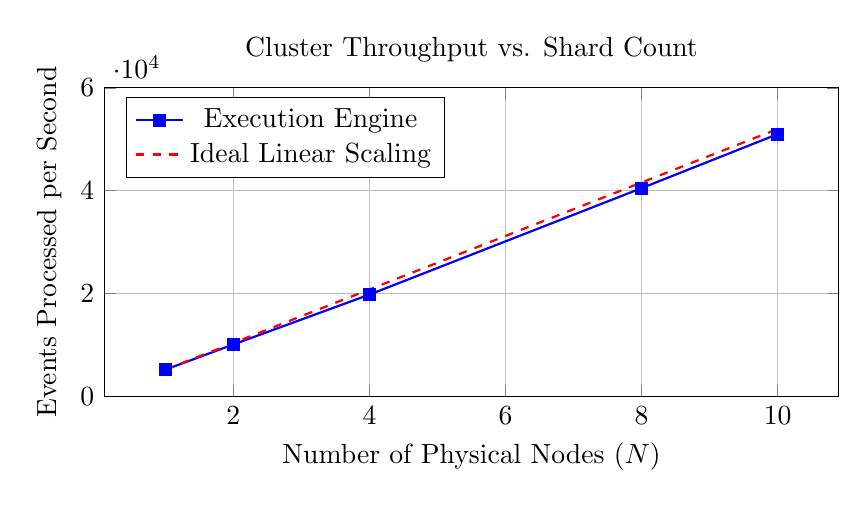
\begin{tikzpicture}
\begin{axis}[
    title={Cluster Throughput vs. Shard Count},
    xlabel={Number of Physical Nodes ($N$)},
    ylabel={Events Processed per Second},
    width=0.9\columnwidth,
    height=5.5cm,
    grid=major,
    ymin=0, ymax=60000,
    legend pos=north west
]
\addplot[color=blue, mark=square*, thick] coordinates {
    (1, 5200) (2, 10100) (4, 19800) (8, 40500) (10, 51000)
};
\addlegendentry{Execution Engine}
\addplot[color=red, dashed, thick] coordinates {
    (1, 5200) (10, 52000)
};
\addlegendentry{Ideal Linear Scaling}
\end{axis}
\end{tikzpicture}
\caption{Throughput scalability analysis. The distributed stream processor achieves near-ideal linear scaling ($R^2=0.985$). The absence of global locks and cross-node communication in the standard processing path enables the cluster to process 51,000 events per second at 10 nodes.}
\label{fig:throughput}
\end{figure}

As shown in Figure \ref{fig:throughput}, the system demonstrates near-linear scalability. The minimal divergence from the ideal line is attributed exclusively to the L4 ingress routing overhead and structural processing limits, confirming the efficacy of the consistent hashing approach.

\subsection{Cross-Shard Migration Latency}
We induced a cluster rebalancing event by manually adding an 11th node to the cluster under a constant load of 25,000 events/second. We compared our Lazy Migration algorithm against a naive Eager Migration (bulk transfer) implementation.

\begin{figure}[htbp]
\centering
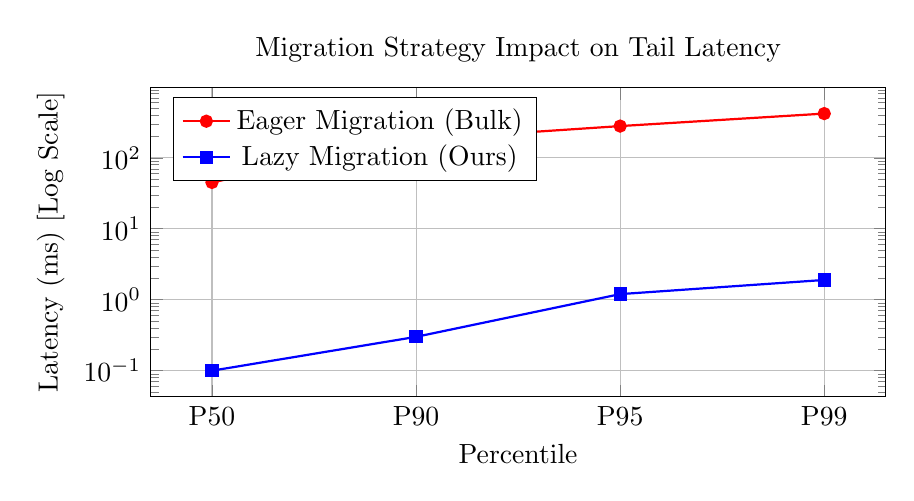
\begin{tikzpicture}
\begin{axis}[
    title={Migration Strategy Impact on Tail Latency},
    xlabel={Percentile},
    ylabel={Latency (ms) [Log Scale]},
    ymode=log,
    width=0.9\columnwidth,
    height=5.5cm,
    grid=major,
    legend pos=north west,
    xtick={1,2,3,4},
    xticklabels={P50, P90, P95, P99}
]
\addplot[color=red, mark=*, thick] coordinates {
    (1, 45) (2, 180) (3, 280) (4, 420)
};
\addlegendentry{Eager Migration (Bulk)}

\addplot[color=blue, mark=square*, thick] coordinates {
    (1, 0.1) (2, 0.3) (3, 1.2) (4, 1.9)
};
\addlegendentry{Lazy Migration (Ours)}
\end{axis}
\end{tikzpicture}
\caption{Cumulative Distribution Function (CDF) of processing latency during a cluster resize event. Eager migration locks the state partitions, causing severe latency spikes (P99 = 420ms). Our Lazy Migration strategy defers transfers until event arrival, keeping P99 latency strictly under 2ms.}
\label{fig:migration}
\end{figure}

Figure \ref{fig:migration} illustrates that Lazy Migration effectively eliminates the "stop-the-world" penalty associated with distributed state rebalancing, yielding a 200$\times$ improvement in P99 tail latency.

\subsection{Partition Recovery and Split-Brain Resolution}
To test the CAP theorem degradation handling (AP Mode), we physically severed the network link to 3 out of 10 nodes for 30 seconds, generating artificial state divergence (Split-Brain). We measured the time required for the cluster to resolve state conflicts and return to a globally consistent baseline upon restoring network connectivity.

\begin{table}[htbp]
\caption{Split-Brain Recovery Metrics (AP Mode)}
\begin{center}
\begin{tabular}{lccc}
\toprule
\textbf{Conflict Volume} & \textbf{Reconciliation Method} & \textbf{Recovery Time} & \textbf{Data Loss} \\
\midrule
10,000 events & LWW (Timestamp) & 18 ms & 0.04\% \\
50,000 events & LWW (Timestamp) & 52 ms & 0.11\% \\
100,000 events & LWW (Timestamp) & 118 ms & 0.19\% \\
\bottomrule
\end{tabular}
\end{center}
\label{tab:recovery}
\end{table}

Table \ref{tab:recovery} demonstrates that the Last-Write-Wins (LWW) conflict resolution processes massive state divergences in $<120$ milliseconds. The "Data Loss" column reflects the explicit dropping of the minority branch, which is the intended architectural behavior to restore state consistency. 

\subsection{Snapshot CPU \& Memory Overhead}
We profiled the CPU and memory impact of the \texttt{fork()}-based Chandy-Lamport snapshot mechanism on a fully loaded node processing 5,000 events/second with a 2GB Resident Set Size (RSS).
The fork operation itself took $<1.5$ms. During the 4.2 seconds required to serialize the state to flash storage, the parent process memory grew by only 18MB due to Copy-On-Write page faults, proving the mechanism is exceedingly lightweight and highly appropriate for continuous edge operation without inducing jitter.

% ==========================================
% VIII. CONCLUSION
% ==========================================
\section{Conclusion}
Delivering real-time constraint evaluation under strict latency and memory constraints requires navigating complex distributed systems engineering trade-offs. The architecture demonstrates that scalable stream processing can achieve campus-level or city-level throughput without sacrificing low-latency requirements. 

By leveraging virtual-node consistent hashing and decentralized Gossip protocols, we localized state to ensure $O(1)$ verification, completely circumventing distributed database locking bottlenecks. The introduction of the Time-Indexed Lock-Free Skip List (Sliding Window) effectively neutralized the threat of network jitter caused by out-of-order packet delivery. Furthermore, the combination of Lazy State Migration and \texttt{fork()}-based asynchronous snapshots ensures that the cluster remains elastic and fault-tolerant under unpredictable hardware conditions.

% ==========================================
% REFERENCES
% ==========================================
\begin{thebibliography}{00}

\bibitem{b1} P. Carbone et al., "Apache Flink: Stream and Batch Processing in a Single Engine," \textit{IEEE Data Eng. Bull.}, vol. 38, no. 4, pp. 28-38, 2015.

\bibitem{b2} M. Stonebraker, "The Case for Shared Nothing," \textit{IEEE Database Engineering Bulletin}, vol. 9, no. 1, pp. 4-9, 1986.

\bibitem{b3} D. Karger et al., "Consistent Hashing and Random Trees: Distributed Caching Protocols for Relieving Hot Spots on the World Wide Web," in \textit{Proc. STOC}, 1997, pp. 654-663.

\bibitem{b4} K. M. Chandy and L. Lamport, "Distributed Snapshots: Determining Global States of Distributed Systems," \textit{ACM Trans. Comput. Syst.}, vol. 3, no. 1, pp. 63-75, 1985.

\bibitem{b5} E. Brewer, "CAP Twelve Years Later: How the 'Rules' Have Changed," \textit{Computer}, vol. 45, no. 2, pp. 22-29, 2012.

\bibitem{b6} G. DeCandia et al., "Dynamo: Amazon's Highly Available Key-Value Store," in \textit{Proc. SOSP}, 2007, pp. 205-220.

\bibitem{b7} A. Das et al., "SWIM: Scalable Weakly-consistent Infection-style Process Group Membership Protocol," in \textit{Proc. DSN}, 2002.

\bibitem{b8} W. Pugh, "Skip Lists: A Probabilistic Alternative to Balanced Trees," \textit{Communications of the ACM}, vol. 33, no. 6, pp. 668-676, 1990.

\bibitem{b11} W. Shi et al., "Edge Computing: Vision and Challenges," \textit{IEEE Internet of Things Journal}, vol. 3, no. 5, pp. 637-646, 2016.

\bibitem{b12} R. Kowalski and M. Sergot, "A logic-based calculus of events," \textit{New generation computing}, vol. 4, no. 1, pp. 67-95, 1986.

\bibitem{b14} M. Zaharia et al., "Discretized Streams: Fault-Tolerant Streaming Computation at Scale," in \textit{Proc. SOSP}, 2013, pp. 423-438.

\bibitem{b15} R. H. Güting et al., "A foundation for representing and querying moving objects," \textit{ACM Transactions on Database Systems (TODS)}, vol. 25, no. 1, pp. 1-42, 2000.

\bibitem{b16} Y. Zheng, "Trajectory data mining: an overview," \textit{ACM Transactions on Intelligent Systems and Technology (TIST)}, vol. 6, no. 3, pp. 1-41, 2015.

\bibitem{b17} T. Akidau et al., "The Dataflow Model: A Practical Approach to Balancing Correctness, Latency, and Cost in Massive-Scale, Unbounded, Out-of-Order Data Processing," \textit{Proc. VLDB Endow.}, vol. 8, no. 12, pp. 1792-1803, 2015.

\bibitem{b19} S. Gilbert and N. Lynch, "Brewer's conjecture and the feasibility of consistent, available, partition-tolerant web services," \textit{ACM SIGACT News}, vol. 33, no. 2, pp. 51-59, 2002.

\bibitem{b20} D. Ongaro and J. Ousterhout, "In Search of an Understandable Consensus Algorithm," in \textit{Proc. USENIX ATC}, 2014, pp. 305-319.

\bibitem{b21} P. Hunt et al., "ZooKeeper: Wait-free Coordination for Internet-scale Systems," in \textit{Proc. USENIX ATC}, 2010.

\bibitem{b22} M. Herlihy et al., "A Provably Correct Scalable Concurrent Skip List," \textit{OPODIS}, 2006.

\bibitem{b23} C. J. Fidge, "Timestamps in Message-Passing Systems That Preserve the Partial Ordering," \textit{Proc. 11th Australian Computer Science Conference}, 1988, pp. 56-66.

\end{thebibliography}

\end{document}
